\section{Potenze e radici complesse}

Per risolvere equazioni nel campo dei complessi (o equivalentemente per fattorizzare polinomi in $\C[x]$) è necessario saper calcolare potenze di numeri complessi e radici $n$-esime.

La forma cartesiana non è particolarmente di aiuto in questo caso: calcolare le potenze è difficile in quanto dovremmo ricorrere costantemente a prodotti tra binomi della forma $a+ib$, mentre calcolare le radici è impossibile a causa della somma tra parte reale e immaginaria.

La forma polare risulta invece molto più comoda, come ci garantisce la seguente proposizione.
\begin{proposition}\label{prop:power_complex}
    Sia $z = \rho e^{i\theta}$ un numero complesso. Allora la sua potenza $n$-esima è \begin{equation}
        z^n = \rho^n e^{in\theta}.
    \end{equation}
\end{proposition}
\begin{proof}
    Lo mostriamo per induzione su $n$.
    \begin{description}
        \item[Caso base] Se $n = 1$ allora \[
            z^1 = (\rho e^{i\theta})^1 = \rho^1 e^{1 \cdot 1\theta}.    
        \] 
        \item[Passo induttivo] Supponiamo la formula valga per $k$ e dimostriamola per $k + 1$.
        \begin{align*}
            z^{k+1} &= z^k \cdot z \tag{per hp. induttiva}\\
            &= \rho^k e^{ik\theta} \cdot \rho e^{i\theta} \tag{per la \autoref{prop:product_polar}}\\
            &= (\rho^k \rho) e^{i(k\theta+\theta)} \\
            &= \rho^{k+1} e^{i(k+1)\theta}.
        \end{align*} 
    \end{description}
    Dunque la formula è vera per ogni valore di $n$, come volevasi dimostrare.
\end{proof}

La potenza $n$-esima di un numero complesso di modulo unitario (diciamo $z = e^{i\theta}$) corrisponde alla rotazione del vettore corrispondente fino ad arrivare al vettore di angolo $n\theta$: equivale infatti a moltiplicare il vettore per se stesso $n$ volte, e ognuna di queste moltiplicazioni ruota il vettore di un angolo di $\theta$ radianti (come abbiamo osservato nella sezione precedente).

Il problema di trovare la radice $n$-esima di un numero è completamente riconducibile al problema di calcolare potenze di numeri complessi. Supponiamo di voler calcolare la radice $n$-esima di un numero complesso $w  \in \C$ dato, ovvero vogliamo trovare $z \in \C$ tale che \begin{equation}
    z = \sqrt[n]{w}.
\end{equation} Riformulando il problema, vogliamo trovare $z \in \C$ tale che \begin{equation}
    z^n = w.
\end{equation}

\paragraph{Caso $w = 1$} Iniziamo studiando un caso più semplice: consideriamo il numero complesso $w = 1$. Nel campo dei numeri reali il numero $1$ ha sempre una e una sola radice, ovvero se stesso. Nei numeri complessi, come vedremo, il numero $1$ ha più di una radice $n$-esima; in particolare, ne ha esattamente $n$.

Sia $z \in \C$ una radice $n$-esima di $1$ ($z = \sqrt[n]{1}$), ovvero equivalentemente sia $z \in \C$ tale che $z^n = 1$. Siccome stiamo calcolando potenze di numeri complessi scriviamo ogni numero in forma polare: il numero $1$ è esprimibile come $1\cdot e^{i0}$; siano inoltre $\rho$ e $\theta$ rispettivamente il modulo e l'argomento di $z$, cosicché $z = \rho e^{i\theta}$. Per la \autoref{prop:power_complex} segue quindi che $z^n = \rho^n e^{in\theta}$.

Come abbiamo osservato alla fine della sezione precedente, due numeri complessi in forma polare sono uguali se e solo se \begin{itemize}
    \item hanno lo stesso modulo;
    \item i loro argomenti differiscono per un multiplo di $2\pi$.
\end{itemize} Applicando questo ragionamento all'equazione $z^n = 1$ (che è l'equazione che definisce $z$) otteniamo due condizioni che possiamo sfruttare per calcolare $z$:
\begin{itemize}
    \item I moduli devono essere uguali, dunque segue che $\rho^n = 1$. Dato che $\rho$ è un numero reale, questa equazione ha una e una sola soluzione: $\rho = 1$.
    \item Gli argomenti devono differire per un multiplo di $2\pi$, ovvero $\arg z - \arg 1 = n\theta - 0 = 2k\pi$ per qualche $k \in \Z$.
\end{itemize} Dal primo vincolo otteniamo $\rho = 1$, mentre dal secondo ricaviamo che $\theta$ deve essere della forma $\dfrac{2k\pi}{n}$, al variare di $k \in \Z$.

Anche se l'equazione sembra avere infinite soluzioni (una per ogni valore di $k$ intero), in realtà le soluzioni distinte sono solo $n$, e si ottengono scegliendo $k = 0, \dots, n-1$. Infatti scegliendo $k = n$ l'argomento di $z$ diventa $\nicefrac{(2n\pi)}{n} = 2\pi = 0$ (poiché gli argomenti rappresentano angoli in radianti), che è lo stesso argomento ottenuto scegliendo $k = 0$.

Le possibili soluzioni dell'equazione $z^n = 1$, e quindi dell'equazione $z = \sqrt[n]{1}$, sono dunque della forma \[
    1\cdot e^{i\frac{2k\pi}{n}}
\] con $k = 0, \dots, n-1$. Questi numeri vengono detti \emph{radici $n$-esime dell'unità} e vengono spesso chiamati $\mu_0, \dots, \mu_{n-1}$.

Rappresentando ad esempio le radici seste dell'unità possiamo notare immediatamente alcune caratteristiche interessanti:
\begin{center}
    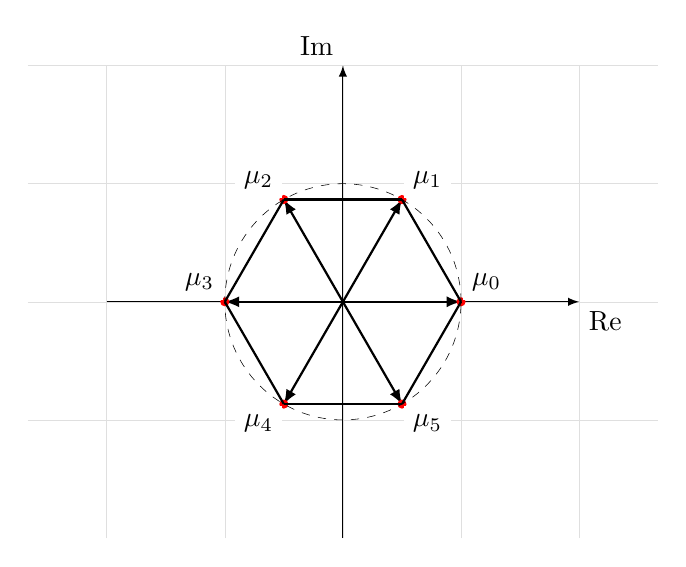
\begin{tikzpicture}[>=latex]
        \coordinate (mu0) at (1.5, 0);
        \draw[step=1.5cm,gray!25!,very thin] (-4,-3) grid (4,3);
        \draw[thin,->] (-3,0) -- (3,0) node[anchor=north west] {Re};
        \draw[thin,->] (0,-3) -- (0,3) node[anchor=south east] {Im};
        \draw[black,thick,->] (0,0) coordinate (O) -- (mu0);
        \draw[black,thick,->] (O) -- (60:1.5) coordinate (mu1);
        \draw[black,thick,->] (O) -- (120:1.5) coordinate (mu2);
        \draw[black,thick,->] (O) -- (180:1.5) coordinate (mu3);
        \draw[black,thick,->] (O) -- (240:1.5) coordinate (mu4);
        \draw[black,thick,->] (O) -- (300:1.5) coordinate (mu5);
        \filldraw [red,very thick] (mu0) circle (1pt)
        node[black,above right,fill=white] {$\mu_0$};
        \filldraw [red,very thick] (mu1) circle (1pt)
        node[black,above right,fill=white] {$\mu_1$};
        \filldraw [red,very thick] (mu2) circle (1pt)
        node[black,above left,fill=white] {$\mu_2$};
        \filldraw [red,very thick] (mu3) circle (1pt)
        node[black,above left,fill=white] {$\mu_3$};
        \filldraw [red,very thick] (mu4) circle (1pt)
        node[black,below left,fill=white] {$\mu_4$};
        \filldraw [red,very thick] (mu5) circle (1pt)
        node[black,below right,fill=white] {$\mu_5$};

        \draw[black,thick] (mu5) -- (mu0);
        \draw[black,thick] (mu0) -- (mu1);
        \draw[black,thick] (mu1) -- (mu2);
        \draw[black,thick] (mu2) -- (mu3);
        \draw[black,thick] (mu3) -- (mu4);
        \draw[black,thick] (mu4) -- (mu5);

        \draw[color=black, very thin,dashed](0,0) circle (1.5);
    \end{tikzpicture}
\end{center}

Siccome l'angolo tra due radici consecutive è sempre di $\frac{\pi}3$ i vertici dei vettori corrispondenti alle sei radici delle unità formano un esagono regolare, inscritto nella circonferenza unitaria: in generale le radici $n$-esimi dell'unità formano un $n$-agono regolare inscritto nella circonferenza unitaria, e $1$ è sempre un vertice di questo $n$-agono.

Inoltre le radici "non-reali" (come ad esempio $\mu_1$, $\mu_2$, $\mu_4$ e $\mu_5$) sono complesse coniugate a coppie, come si vede evidentemente dal disegno nel caso $n = 6$.